\documentclass[../../Main.tex]{subfiles}

\begin{document}
    \begin{figure}[hbt!]
        \centerline{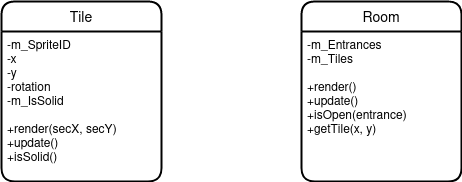
\includegraphics[scale=0.5]{img/Classes/Rooms.png}}
        \caption{Classes for the design of the maze}
        \label{fig}
    \end{figure}
    Tile
    \begin{center}
        Variables
        \begin{tabular}{ | m{0.45\textwidth} | m{0.45\textwidth} | }
            \hline
            \textbf{Variable Name} & \textbf{Description} \\
            \hline
            m\_SpriteID & Stores the sprite ID of the tile \\
            \hline
            x & Stores the x axis relative to the room it is located in \\
            \hline
            y & Stores the y axis relative to the room it is located in \\
            \hline
            rotation & Stores the rotation of the tile \\
            \hline
            m\_IsSolid & Stores whether it is solid or not \\
            \hline
        \end{tabular}
        Functions
        \begin{tabular}{ | m{0.15\textwidth} | m{0.35\textwidth}| m{0.4\textwidth} | }
            \hline
            \textbf{Function Name} & \textbf{Parameters} & \textbf{Description} \\
            \hline
            render & The x and y coordinates of the room it is in & Renders the tile \\
            \hline
            update & & Updates the tile (This is not really used as I do not have any animated tiles) \\
            \hline
            isSolid & & Returns m\_IsSolid \\
            \hline
        \end{tabular}
    \end{center}
    Room
    \begin{center}
        Variables
        \begin{tabular}{ | m{0.45\textwidth} | m{0.45\textwidth} | }
            \hline
            \textbf{Variable Name} & \textbf{Description} \\
            \hline
            m\_Entrances & Stores the entrances and whether they are open or not\\
            \hline
            m\_Tiles & Stores all the tiles as a grid \\
            \hline
        \end{tabular}
        Functions
        \begin{tabular}{ | m{0.15\textwidth} | m{0.35\textwidth}| m{0.4\textwidth} | }
            \hline
            \textbf{Function Name} & \textbf{Parameters} & \textbf{Description} \\
            \hline
            render & & Renders all the tiles \\
            \hline
            update & & Updates the room \\
            \hline
            isOpen & Entrance (this is its own type) & returns whether an entrance is open \\
            \hline
            getTile & x and y position & Returns a tile at the give coordinates \\
            \hline
        \end{tabular}
    \end{center}
\end{document}